\documentclass{article}


% load package with some of the available options - you may not need this!
\usepackage[framed,autolinebreaks,useliterate]{mcode}

% for checklist
\usepackage{enumitem,amssymb}
\newlist{todolist}{itemize}{2}
\setlist[todolist]{label=$\square$}
\usepackage{pifont}
\newcommand{\cmark}{\ding{51}}%
\newcommand{\xmark}{\ding{55}}%
\newcommand{\done}{\rlap{$\square$}{\raisebox{2pt}{\large\hspace{1pt}\cmark}}%
\hspace{-2.5pt}}
\newcommand{\wontfix}{\rlap{$\square$}{\large\hspace{1pt}\xmark}}


% something NOT relevant to the usage of the package.
\usepackage{graphicx}
\usepackage{url,textcomp}
\setlength{\parindent}{0pt}
\setlength{\parskip}{18pt}
\title{ECTA Homework 1\\Genetic Algorithms\\and\\Infinite Monkeys}
\author{\color{red} Debaraj Barua (9030412), \texttt{debaraj.barua@smail.inf.h-brs.de} \\
\color{red}Md Zahiduzzaman (9030432), \texttt{md.zahiduzzaman@smail.inf.h-brs.de}}
% //////////////////////////////////////////////////

\begin{document}

\maketitle

\begin{center}
\begin{minipage}{1\linewidth}
	\begin{center}
    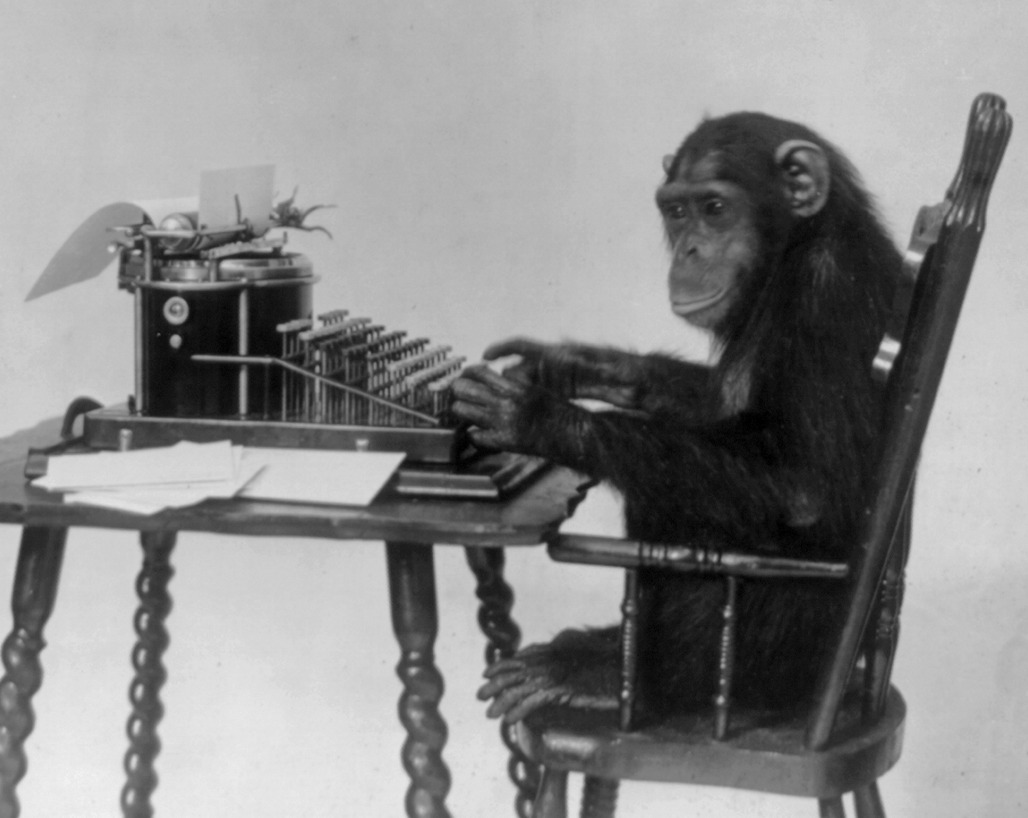
\includegraphics[width=0.75\textwidth]{img/chimp}  
    \end{center}
    
	{\large The infinite monkey theorem states that if a chimpanzee hits keys at random on a typewriter for an infinite amount of time, it will eventually type the complete works of William Shakespeare. Is this what evolution is doing? It has been argued that the genetic mutations required to move from a single cell to multicellular life are as unlikely as a monkey typing Hamlet's soliloquy. But is evolution just a monkey banging on a typewriter?}	
\end{minipage}
\end{center}

\section{Assignment Description}
	\begin{enumerate}
		\item Build a simple Genetic Algorithm and test the effect of each component
		\begin{itemize}
			\item Mutation
			\item Crossover
			\item Elitism		
		\end{itemize}
		\item Answer the question, "is evolution just a monkey banging on a typewriter?"	
	\end{enumerate}

	\begin{itemize}
  	\item Grading Scheme
  		\begin{todolist}
  		\item Code a GA (40 pts)
  			\begin{todolist}
  			\item Selection (10pts)
  			\item Crossover (10pts)
  			\item mutation 	(10pts)
  			\item Elitism 	(10pts)
  			\end{todolist}
  		\item GA Component Comparisons (40 pts)
  		  	\begin{todolist}
  			\item Comparison vs. Standard Implementation (5 pts)
  			\item Comparison of Components (5 pts)
  			\item Short Answer \#1 (10 pts)
  			\item Short Answer \#2 (10 pts)
  			\item Short Answer \#3 (10 pts)
  			\end{todolist}
  		\item GA vs Monkey (20 pts)
  		  	\begin{todolist}
  			\item Solve the soliloquy 		(10 pts)
  			\item Brute force calculation 	(5 pts)
  			\item Short Answer \#4 			(5 pts)
  			\end{todolist}
  		\end{todolist}
	\end{itemize}
\newpage


\section{Submission Instructions}
Follow along with the instructions in this PDF, filling in your own code, data, and observations as noted. Your own data should be inserted into the latex code of the PDF and recompiled. All code must be done in MATLAB. The basic structure of the code and fitness function are provided, but all code should be submitted as a separate zipped file in LEA. Relevant sections of code can be inserted directly into this document using the mcode latex package. This package is attached with documentation, and in this document I have provided usage examples.

To be perfectly clear we expect two submissions to LEA:
\begin{enumerate}
	\item 1 PDF (report) -- a modified version of this PDF, with your own code snippets, figures, and responses inserted
	\item 1 ZIP (code and data)   -- a .zip file containing all code use to run experiments (.m files) \textit{and} resulting data as a .mat file
\end{enumerate}

\newpage

\section{Assignment Overview}
\subsection*{the Task}
Like our monkey, your Genetic Algorithm will be tested as to how closely it can reproduce Shakespeare. Two benchmarks are given: \mcode{hamletQuote} and \mcode{hamletSoliloquy}. These functions take one or more genes of length 18 for the quote or 1446 for the soliloquy and return a fitness value which corresponds to the number of letters that match the target text.

One gene is a number between 0 and 27, corresponding to a space (0), letters a-z (1-26), and a new line (27).

\subsection*{the Algorithm}
I have created the basic structure of the GA for you. The magic happens in the loop here in \mcode{monkeyGa.m}:

\lstinputlisting[firstline=88, lastline=107]{../code/monkeyGa.m}

It will be your job to implement each of the evolutionary operators and measure how they effect performance of the algorithm on the \mcode{hamletQuote} task. 

\subsection*{Running the Algorithm}
	To run the algorithm and view the results, you can use the snippet provided at the start of \mcode{monkeyExperiment.m}:

\lstinputlisting[firstline=1, lastline=11]{../code/monkeyExperiment.m}

	To run a section in matlab (a code block marked by \mcode{\%\%}, with the cursor inside the code block click the `Run Section' button in the editor portion of the ribbon, or more simply hit `CTRL + Enter'). Run it a few times. As the only operator which is implemented is initialization, it will give you a pretty terrible result.

\subsection*{Comparing Algorithms}
As evolutionary algorithms are based on stochastic processes, they will not perform the same every time. Whenever a comparison between two algorithms or algorithm settings is made, it \emph{must} be a comparison over several runs. Comparisons between runs must take into account the effect of randomness, including significance of results (how likely the result is to be because of chance).

\newpage
\section{The Assignment}

\subsection{Coding a simple GA}
Begin by implementing the four given genetic operators, replacing the filler code with your own. The expected inputs and outputs, as well as hints as how to perform each operation are included within the code. Please put your code in the report here using the given `firstline/lastline' syntax in the \LaTeX.\\ \textit{Don't overthink it! Each of these can be done in less than 10 lines!}
\begin{enumerate}
%-------------------------%
% Put your code here:

\item \textbf{Tournament Selection}
	\lstinputlisting[firstline=30, lastline=45]{../code/my_selection.m}
	
\item \textbf{Crossover}
	\lstinputlisting[firstline=29, lastline=52]{../code/my_crossover.m}
	
\item \textbf{Mutation}
	\lstinputlisting[firstline=24, lastline=42]{../code/my_mutation.m}
	
\item \textbf{Elitism}
	\lstinputlisting[firstline=27, lastline=33]{../code/my_elitism.m}	
	
%-------------------------%
\end{enumerate}


\subsection{Ablation Study}
One common technique for better understanding an algorithm is remove each component and see the result. What happens when we don't use elitism or we skip crossover? In this section we test a few combinations. 

\subsubsection{Comparing Algorithms}
Provided are versions of each operator with the prefix `adam' instead of `my'. These can be used to validate your own results. I included a version which uses them in the file `adamGa', which is exactly the same except this part:

	\lstinputlisting[firstline=90, lastline=100]{../code/adamGa.m}

As this is a stochastic algorithm to get a fair comparison we should run the algorithm multiple times and compare statistically. Lets use all the cores on your computer to do this as fast as possible using a \mcode{parfor} loop. This is just like a \mcode{for} loop, except it runs each iteration on a different core. Get the result of 20 runs of your code and mine and save it to disk:

	\lstinputlisting[firstline=16, lastline=29]{../code/monkeyExperiment.m}

With this data saved you can compare the two algorithms and compute the significance of the comparison. I have given you a few helper functions:

	\lstinputlisting[firstline=45, lastline=64]{../code/monkeyExperiment.m}

	\begin{figure}[h!]
	\begin{center}
	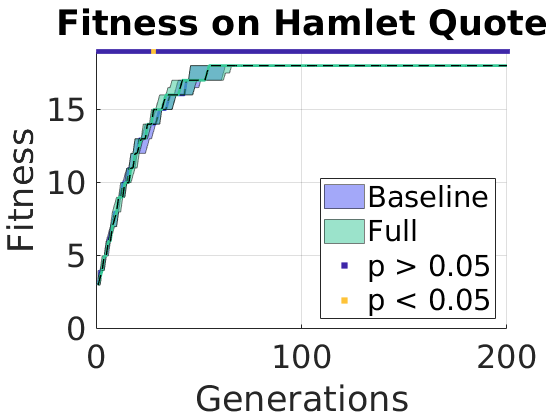
\includegraphics[width=0.75\textwidth]{img/1_vsStandard_my.png}
	\caption{\color{red}Baseline vs Full}
	\end{center}
	\end{figure}
	
	This plot shows the median performance at each generation (dashed lines) of each algorithm along with their upper and lower quartiles. Indicated at the top is the probability that the two algorithms are the same. Unsurprisingly, both runs of the same algorithm are statistically the same. Replace this plot with one of your own creation, comparing my code with your own implementation, to ensure that your code is working.
\newpage
	Perform the following comparisons of your algorithm with various components removed and replace the plots with your own, this can be done by replacing the functions in the code and saving the result (e.g. replacing the \mcode{my_crossover} function with the \mcode{no_crossover} function: (1) Your full implementation vs. No crossover, (2) Your full implementation vs. No mutation, (3) No crossover vs. No crossover AND no elitism, and (4) No mutation  vs. No mutation AND no elitism.

		\begin{figure}[h!]
		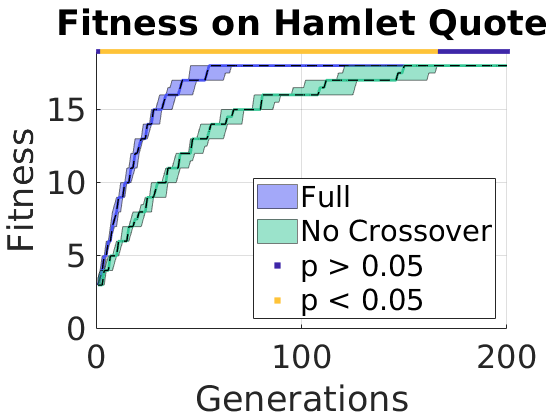
\includegraphics[width=0.5\textwidth]{img/2_vsNoCross_my.png}
		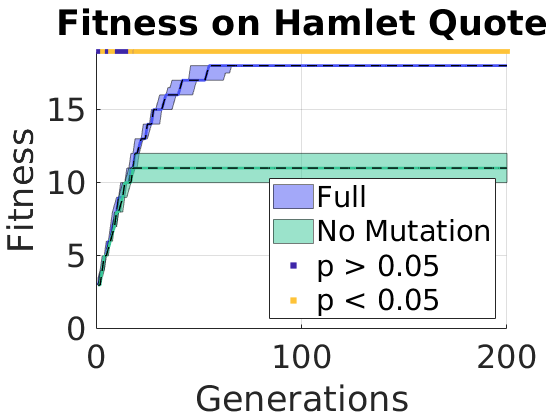
\includegraphics[width=0.5\textwidth]{img/3_vsNoMut_my.png}
		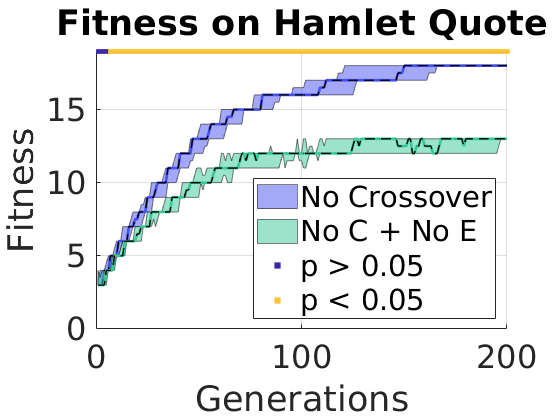
\includegraphics[width=0.5\textwidth]{img/4_vsNoCrossNoElite_my.png}
		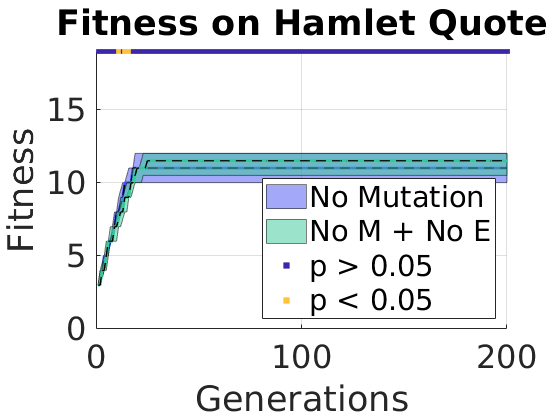
\includegraphics[width=0.5\textwidth]{img/5_vsNoMutNoElite_my.png}
		\caption
		{
		\textbf{GA performance when operators are removed}\newline
		\textit{Top Left:} No Crossover,
		\textit{Top Right:} No Mutation, 
		\textit{Bottom Left:} No Crossover vs. No Crossover and No Elitism, 
		\textit{Bottom Right:} No Mutation and No Elitism
		\color{red}FILL IN YOUR OWN PLOTS HERE
		}
		\end{figure}
\newpage
\subsubsection{Analyzing the Results}
\begin{enumerate}
	\item \textbf{Describe the main purposes of crossover and of mutation, how do your results illustrate their operation?} \\
%-------------------------%
% ANSWER: 
\textit{
 \color{red}WRITE SOMETHING HERE
 }
%-------------------------%

	\item \textbf{When only crossover is used the problem is not typically solved. Why? Could you devise an experiment that would support your explanation? One in which crossover could the solve the problem every time?}\\
%-------------------------%
% ANSWER:
\textit{
\color{red}WRITE SOMETHING HERE
 }
%-------------------------%
	
	\item \textbf{Describe the benefits of elitism in the crossover and mutation only cases.}\\
%-------------------------%
% ANSWER:
\textit{
\color{red}WRITE SOMETHING HERE
}
%-------------------------%	

\end{enumerate}

\newpage
\subsection{Monkeys on a Typewriter}
\subsubsection{Using the GA}
Now time to test your algorithm on the entire soliloquy. Is it really better than just banging on a typewriter? Switch out the fitness function and give the whole speech a try. It might take a little time, you may have to increase the number of generations to get to 100\%, for this purpose don't worry about replicates:

\lstinputlisting[firstline=67, lastline=76]{../code/monkeyExperiment.m}

By using the \mcode{tic} and \mcode{toc} commands we can time how long a program takes to execute. How long did it take your algorithm to find the whole speech?\\
%-------------------------%
% ANSWER:
\textit{
\color{red}WRITE SOMETHING HERE
}
%-------------------------%	

\newpage
\subsubsection{Brute force}
How long would it take to find the same solution by a monkey on a type writer, i.e. by brute force? The average and worst case for a brute force algorithm can be easily calculated by counting the possible states. Let's be charitable and say this is a particularly clever monkey, who is systematic and never typing the same thing twice. Lets be even more charitable and say that this clever monkey also has a MATLAB license and has created a program to do the typing for him. How many possible states are there? How long will it take this MATLAB monkey to explore them all? Please show your work and use appropriate units for your answer.

(hint: to time a very fast piece of code, repeat in many times and take the average time, like this: )
\lstinputlisting[firstline=83, lastline=88]{../code/monkeyExperiment.m}


%-------------------------%
% ANSWER:
\textit{
\color{red}WRITE SOMETHING HERE
}
%-------------------------%

\vspace{3cm}
How comparable are these methods? Is random search comparable to evolutionary search?\\
%-------------------------%
\textit{
\color{red}WRITE SOMETHING HERE
}
%-------------------------%	






\newpage
\section{Inserting MATLAB code into LATEX --- 3 ways}

1) This inline demo \mcode{for i=1:3, disp('cool'); end;} uses the \verb|\mcode{}| command.\footnote{Works also in footnotes: \mcodefn{for i=1:3, disp('cool'); end;}}

2) The following is a block using the \verb|lstlisting| environment.
\begin{lstlisting}
for i = 1:3
	if i >= 5 && a ~= b       % literate programming replacement
		disp('cool');           % comment with some §\mcommentfont\LaTeX in it: $\mcommentfont\pi x^2$§
	end
	[:,ind] = max(vec);
	x_last = x(1,end) - 1;
	v(end);
	really really long really really long really really long really really long really really long line % blaaaaaaaa
	ylabel('Voltage (µV)');
end
\end{lstlisting}
Note: Here, the package was loaded with the \verb|framed|, \verb|numbered|, \verb|autolinebreaks| and \verb|useliterate| options.  \textbf{Please see the top of mcode.sty for a detailed explanation of these options.}


3) Finally, you can also directly include an external m-file from somewhere on your hard drive (the very code you use in \textsc{Matlab}, if you want) using the \verb|\lstinputlisting{/SOME/PATH/FILENAME.M}| command.  If you only want to include certain lines from that file (for instance to skip a header), you can use \verb|\lstinputlisting[firstline=6, lastline=15]{/SOME/PATH/FILENAME.M}|.


\end{document}